
\item A ball of radius \( R = 10.0\ cm \) rolls without slipping down an inclined plane so that its centre moves with constant acceleration
    \begin{center}
        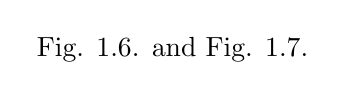
\begin{tikzpicture}
            \node at (0, 0) {Fig. 1.6. and Fig. 1.7.};
            % Diagrams should be drawn here according to the actual diagrams in the image provided
        \end{tikzpicture}
    \end{center}
    \begin{enumerate}
        \item \( w = 2.50\ cm/s^2; \quad t = 2.00\ s \) after the beginning of motion its position corresponds to that shown in Fig. 1.7. Find: the velocities of the points \( A, B, \) and \( O; \)
        \item the accelerations of these points.
    \end{enumerate}
